\part{Complex meshes}
\frame{\partpage}

\begin{frame}{Mesh Formats}
	\begin{itemize}
		\item Typically we invent our own mesh format (see Doom's MD6, Valve's smd formats)
		\pause\item These formats are optimised for realtime rendering and are very efficient
		\pause\item Usually developers write exporters for Maya or 3DSMax to support their format
		\pause\item We are going to use FBX (Autodesk Filmbox) as our model format, this known as an 'interchange' format
	\end{itemize}
\end{frame}

\begin{frame}{Quick Tour of the FBX Format}
	\begin{center}
		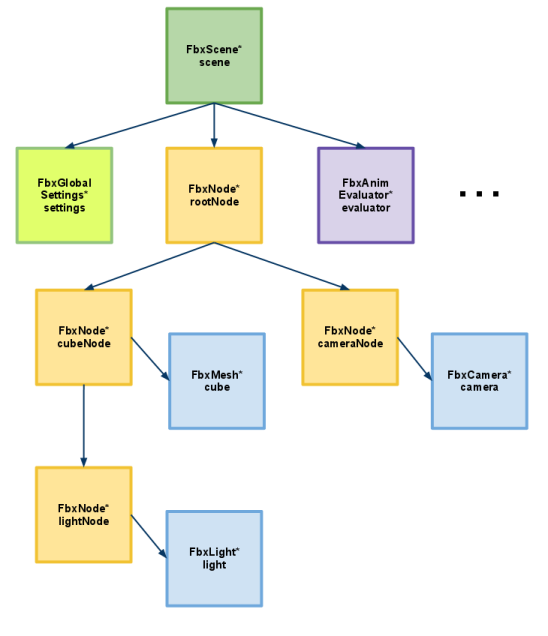
\includegraphics[width=\textwidth,height=0.8\textheight]{scene_org}
	\end{center}
\end{frame}